\documentclass{article}

\title{Trabalho de Graduação\n Sistema de  Verificação de Medicamento em UTI}
\author{}

\usepackage[margin=0.8in]{geometry}
\usepackage{indentfirst}
\usepackage{fancyhdr}
\usepackage{tcolorbox} 
\usepackage{graphicx}
\usepackage{amsmath}
\usepackage{amssymb}
\usepackage{enumitem}
\usepackage{tabularx} % in the preamble
\usepackage{wrapfig}
\usepackage{subcaption}
\usepackage{caption}
\usepackage{listings}
\usepackage{tikz}
\usepackage{multirow}
\usepackage{cancel}
\usepackage{multicol}
\usepackage{float}


% Create a Todo list
\newlist{todolist}{itemize}{2}
\setlist[todolist]{label=$\square$}

% Fix vspace inside wrapfigure
\setlength\intextsep{0pt}

\newcolumntype{Y}{>{\centering\arraybackslash}X}

\captionsetup[lstlisting]{skip=10pt}

% Create a new command to be used in the align environment in multiple line equations do only the last equation is numbered  
\newcommand{\n}{\nonumber \\ }
\makeatletter
\let\inserttitle\@title
\makeatother
% Set the style of the page 
\pagestyle{fancy}
\fancyhf{}
\rhead{Trabalho de Graduação \\ Pedro Henrique L. da Cruz \vspace{1px}}
\lhead{UNICAMP \\ Faculdade de Engenharia Mecânica\vspace{1px}}
\rfoot{Page \thepage}

\usepackage{hyperref}
\hypersetup{
    colorlinks=true,
    linkcolor=black,
    filecolor=file,
    urlcolor=black,
    citecolor=black
}

\usepackage{biblatex}
\addbibresource{biblography.bib}

\renewcommand*\contentsname{Sumário}

% Begin the Document 
\begin{document}

    \thispagestyle{empty}
    \begin{center}
    
        \begin{minipage}{0.12\textwidth}
            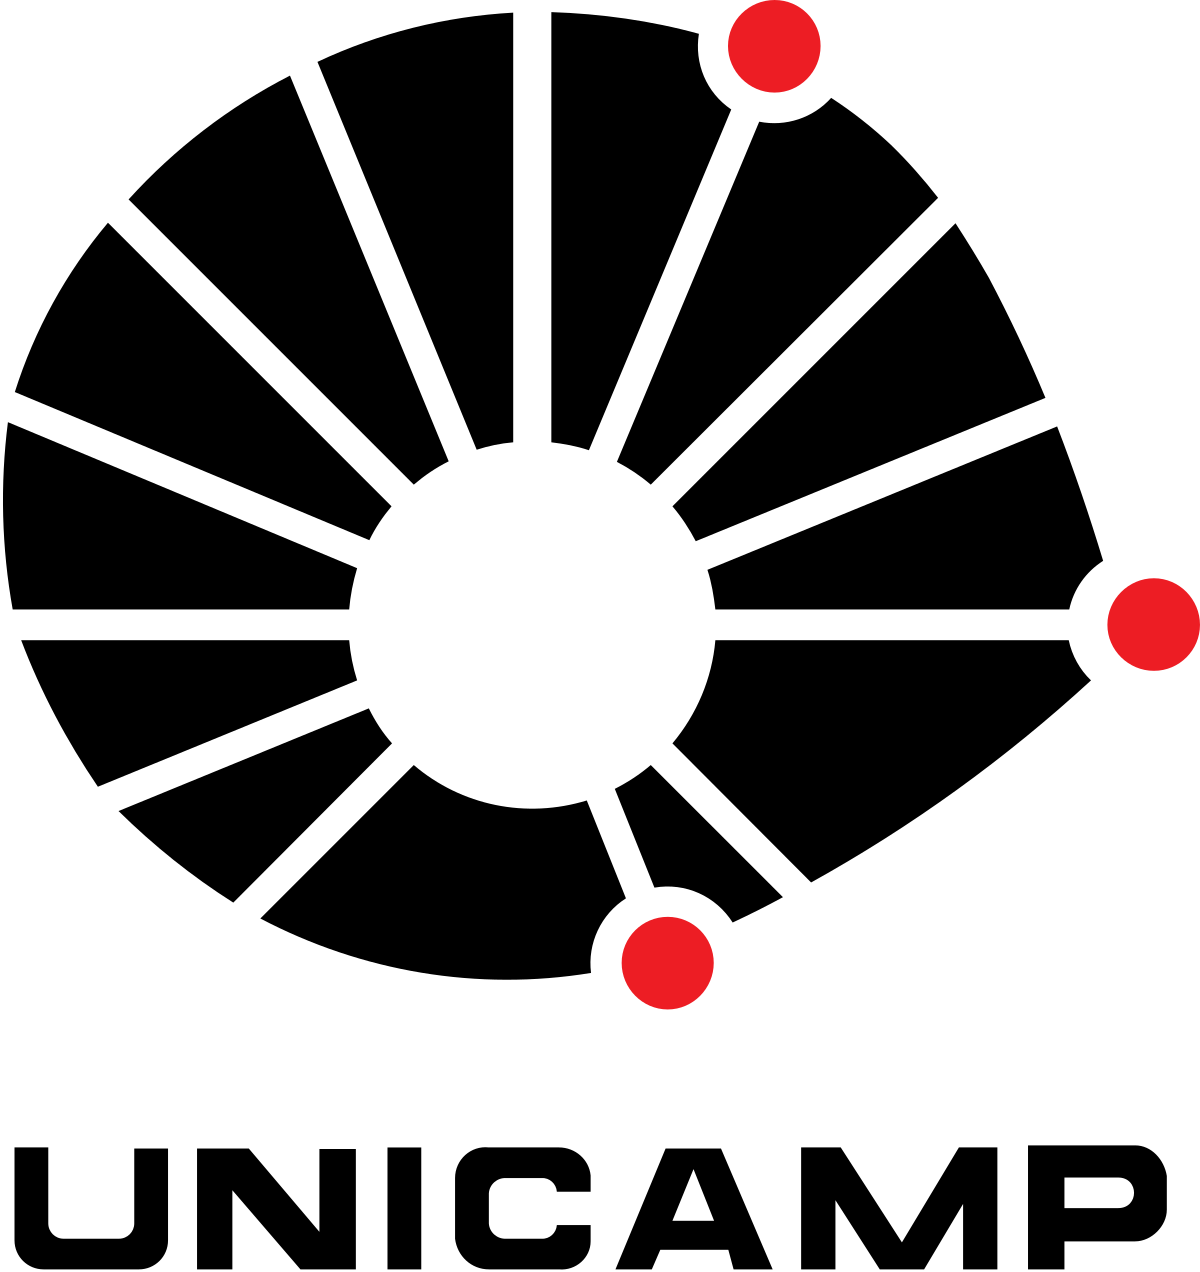
\includegraphics[width=1.5cm]{img/UNICAMP_logo.png} 
        \end{minipage}
        \begin{minipage}{0.50\textwidth}
            \begin{center}
                \textbf{Universidade Estadual de Campinas - UNICAMP} \\
                \textbf{Faculdade de Engenharia Mecânica - FEM}
            \end{center}
        \end{minipage}
        \begin{minipage}{0.15\textwidth}
            \hspace{15px}
            
\includegraphics[width=1.5cm]{img/fem_logo.png} \\
        \end{minipage}
        
    \end{center}

% Title
\vspace{2cm}
\begin{center}
    \textbf{Análise Formal de Controladores PID e Filtros de Média Móvel em C}
\end{center}

% Subtitle
\vspace{1cm}
\begin{center}
    \textbf{Trabalho de Graduação}
\end{center}

% Supervisor and student
\vspace{2cm}
\begin{center}
    \begin{tabular}{l l}
        Orientador: & Prof. Dr. Rodrigo Moreira Bacurau \\
        E-mail: & bacurau@unicamp.br \\
        Aluno: & Pedro Henrique Limeira da Cruz \\
        E-mail: & p215663@dac.unicamp.br
    \end{tabular}
\end{center}

% Date
\vfill{}
\begin{center}
    Campinas, 23 de Fevereiro de 2025.
\end{center}

\newpage
\tableofcontents
\newpage
\section{Introdução}
    \subsection{Motivação}
    Na sociedade atual, a tecnologia está profundamente integrada no cotidiano das pessoas e tornou-se essencial para o funcionamento de diversos setores, incluindo: Saúde, Comunicação, Transporte e Segurança. 
    Em muitos casos, o desempenho correto das funções atribuídas a esses sistemas tecnológicos é crucial, pois sua falha tem repercussões catastróficas, como a perda de vidas, desastre ambientais e prejuízos econômicos. Sistemas com tais responsabilidades são  categorizados como \emph{Safety-Critical}. 

    Com o passar dos anos, observa-se, também, um aumento cada vez maior da transição desses sistemas de analógicos para o digitais, onde o software tem parte fundamental (com um exemplo sendo o desenvolvimento da aeronave Boeing 787, onde houve um aumento de 8-10 vezes no número de linhas de código quando comparados com o desenvolvimento do seu predecessor o Boeing 777 \cite{do178cguide}). Diante dessa realidade, a necessidade de práticas robustas de Verificação e Validação (V\&V) no ciclo de desenvolvimento de softwares considerados criticos se torna evidente.

    Cada setor da indústria possui seus respectivos \emph{standards} e meios de certificar a completude, corretude, robustez e segurança dos softwares desenvolvidos (e.g. DO-178 para software embarcado aeronáutico e IEC 62304 para software embarcados médico), mas uma característica comum para todos é o elevado nível de complexidade, com autores já questionando a validade dos métodos tradicionais de V\&V para o futuro \cite{rushby2011}, e os altos custos de realizar tais atividades (com projetos podendo gastar até 7 vezes mais em atividades de verificação quando comparados a qualquer outra atividade de desenvolvimento \cite{cofer2012}).

    Como alternativa aos métodos tradicionais de verificação, a Verificação Formal tem ganhado espaço como uma abordagem complementar para garantir a confiabilidade de sistemas críticos. Na indústria aeronáutica, essa técnica foi oficialmente incorporada na revisão mais recente da DO-178C, levando à criação da DO-333. Esse documento detalha quais objetivos de verificação podem ser alcançados por meio de métodos formais, fornecendo diretrizes para sua aplicação na certificação de software embarcado. Grandes empresas do setor, como Airbus e Dassault Aviation, já adotaram essa abordagem em alguma capacidade \cite{cofer2012}\cite{delmas2012}, reconhecendo seu potencial para aumentar a segurança, reduzir custos e melhorar a eficiência do processo de desenvolvimento.

    O termo Verificação Formal refere-se a diferentes métodos matemáticos utilizados para  a especificação, desenvolvimento e verificação de softwares e sistemas digitais \cite{rtca333}, possibilitando a verificação de propriedades de forma automática e exaustiva. A DO-333 separa os métodos de verificação formal em três categorias: \emph{Deductive Methods}, \emph{Model Checking} e \emph{Abstract Interpretation}, sendo os mais promissores aqueles que se encaixam nos métodos dedutivos. 

    Considerando esse contexto, propõe-se neste trabalho a verificação por métodos formais da implementação em C de um controlador PID e de um filtro de média móvel, através de ferramentas open-source (Frama-C e seus diferentes \emph{plugins}), garantindo então a ausência de \emph{Run Time Errors} e a corretude funcional de tais algoritmos.


    \subsection{Objetivos}
    Propõe-se neste trabalho, a verificação formal dos algoritmos do controlador PID e filtro de média móvel, garantindo sua  corretude funcional e a ausência de \emph{runtime errors}. Para tal, será feita:
    \begin{itemize}
        \item A analise do código fonte dos algoritmos, e a identificação de possíveis fontes de \emph{run-time errors} através do \emph{plugin} RTE.
        \item A definção de invariantes e variantes de \emph{loop}, além de \emph{bounds} para os argumentos das funções do \emph{kernel} a fim de sanar todos os Verification Cases gerados pelo \emph{plugin} RTE, garantindo então a ausência de \emph{run-time errors}.
        \item A escrita dos contratos formais, utilizando a linguagem ACSL, das funções analisadas.
        \item A Verificação da corretude funcional das funções através do \emph{pluging} EVA e WP.
    \end{itemize}

    \subsection{Estrutura do Trabalho}
        Este trabalho é organizado da seguinte forma:  Na seção \ref{chap:revisao_teorica} é apresentada uma breve revisão da teoria de métodos formais (fundamento da verificação formal) e alguns conceitos importantes para a área de engenharia de software, provendo assim uma base para o entendimento dos métodos e resultados encontrados; Na seção \ref{chap:projetos_correlatos} são apresentados projetos correlatos, a fim de demonstrar a utilização da verificação formal em diferentes contextos, além das atuais limitações e desafios da sua implementação; A seção \ref{chap:metodologia} abrange as etapas necessárias para a verificação formal, explorando a certificação da corretude funcional e ausência de erros em tempo de execução; A seção \ref{chap:resultados}, por fim, apresenta os resultados das verificações feitas, assim como os desafios e métodos alternativos utilizados para supera-los.


\clearpage
\section{Conceitos e Fundamentação Teórica}\label{chap:revisao_teorica}
    Nesta seção, são apresentados alguns conceitos fundamentais do campo de engenharia de software, como corretude funcional e erros em tempo de execução, em seguida são introduzidas teorias fundamentais para a área de verificação formal, como lógica de Hoare e pré-condição mais fraca, e por fim conceitos de engenharia de controle de sistemas, como controlador PID e filtros. 
    
\subsection{Corretude Funcional}

    Quando nos referimos a corretude funcional de um software, estamos nos referindo à expectativa de que o programa escrito se comporta como o desenvolvedor e os \emph{stakeholders} esperam \cite{kosmatov2024guide}. A fim de ter uma garantia de que o sistema criado possui tal característica, diferentes métodos, com diferentes níveis de complexidade e garantia, podem ser empregados.
    
     Durante o processo de desenvolvimento tradicional de software, tal tipo de verificação é feita através de testes, nos quais entradas, julgadas serem representativas das encontradas durante a operação do software em campo, são utilizadas e as saídas verificadas \cite{blanchard2020introduction}. O problema, entretanto, é que não é factível o desenvolvimento de testes que abrangem todas as possibilidades e combinações de \emph{inputs}, resultando, então, em uma limitação dos testes descrita por Dijkstra: ``Testes são capazes de demonstrar a presença de erros, mas nunca sua ausência" \cite{dijkstra1970ewd249}.
     
    Uma alternativa aos métodos tradicionais é a verificação formal, que tem como objetivo garantir, por meio de provas formais e matemáticas, baseadas na chamada Lógica de Hoare e na regra de pré-condição mais fraca (que serão abordadas mais a frente), que o software se comporte conforme especificado para qualquer entrada válida, ou seja, que respeite as especificações estabelecidas \cite{blanchard2020introduction}. 


\subsection{Erros em Tempo de Execução}
    Erros em tempo de execução, como o nome sugere, são erros que ocorrem somente durante o funcionamento do software e que podem resultar desde comportamentos errôneos do sistema até, no pior dos casos, problemas fatais e não recuperáveis, como o ocorrido no voo inaugural do foguete Ariane 5 \cite{ariane_5_report}. 
    Diferentes erros se enquadram nessa categoria, sendo alguns deles: Divisão por zero, \emph{overflow} e \emph{underflow} de inteiros, \emph{overflow} de números com ponto flutuante, acesso inválido à memória (ponteiros nulos) e acesso fora dos limites de um \emph{array}.
    Devido ao potencial catastrófico que esses tipos de erros possuem, a garantia  de sua ausência é um foco importante no desenvolvimento de sistemas críticos. 
    
    Analogamente à corretude funcional, testes podem ser utilizados em certo nível, mas como uma cobertura total não é possível, não há garantias de corretude \cite{kaestner2010astree}. Por esse motivo, métodos formais têm sido utilizados, dentre esses destaca-se a análise estática baseada em semântica formal, também conhecida como \textit{interpretação abstrata}. Essa abordagem permite derivar garantias mesmo em projetos de grande porte, ao calcular superaproximações seguras da semântica do programa por meio da análise  abstrata do código, cobrindo todos os possíveis comportamentos de execução, de forma conservadora, isso é, quando a ferramenta detecta um possível erro, pode ser um erro real ou apenas uma precaução (falso positivo), mas quando nenhum erro é apontado, há uma garantia formal de que aquele tipo de falha está ausente no código analisado \cite{kaestner2010astree}.
    
    
\subsection{Lógica de Hoare}

Programação de computadores é uma ciência exata e, portanto, todas as propriedades e consequências de sua execução em qualquer cenário podem, a priori, serem determinadas a partir do código em si puramente através de métodos dedutivos, regras definidas de inferência e axiomas \cite{hoare1969axiomatic}. 

Visando fornecer uma base lógica e formal para tal análise de propriedades de programas (sendo uma as mais importantes o seu funcionamento correto e esperado), Hoare propôs, em 1969, uma série de axiomas e regras escritas utilizando a notação chamada de “Tripla de Hoare", que possui, de forma geral, a seguinte estrutura:

\begin{align}
    P \ \  \{C\} \ \ Q
\end{align}

Essa notação deve ser lida como: “Se a condição \( P \) (chamada de pré-condição) é verdadeira antes da execução do comando \( C \), então a condição \( Q \) (chamada de pós-condição) será verdadeira após a execução de \( C \), desde que o programa termine.”

A partir dessa notação, é possível expressar uma série de axiomas e regras de inferência, que servem de alicerce para a análise de programas. 

\subsubsection{Axioma da Atribuição}

O primeiro axioma definido é o que descreve a ação mais simples e corriqueira em programas: A atribuição de um valor para uma variável. Mais especificamente, ele descreve a alteração no estado do programa quando uma instrução de atribuição (como a descrita pela Equação \ref{eq:atribuicao}) é efetuada.

\begin{align}
    x := E
    \label{eq:atribuicao}
\end{align}

O axioma da atribuição é definido por:
\begin{align}
    P(f) \ \  \{x := f\}  \ \ P(x)
\end{align}

O axioma estabelece que, para que uma propriedade \( P \) seja válida após a execução da instrução sobre $x$ (nesta equação representada por $P(x)$), ela deve ser válida com \( f \) substituindo todas as ocorrências de \( x \) na expressão original ($P(f)$), antes da atribuição ocorrer. Isso mostra que realmente $x$ assumiu o valor de $f$.

\subsubsection{Regra de Consequência}

Além de axiomas, é necessário pelo menos uma regra de inferência, a fim de permitir a dedução de novas provas e teorias a partir de axiomas e provas já provadas \cite{hoare1969axiomatic}. 

Uma regra que se encaixa nessa categoria é a regra da consequência, que tem o formato: "Se o código C, a partir de uma pré-condição P, resulta em R, e temos que R implica em S, podemos afirmar que o mesmo código e pré-condição implicam em S". Formalmente descrita por:

\begin{align}
    P \ \ \{C\} \ \ R, \ \ R \Rightarrow S \ \ \therefore P \ \ \{C\} \ \ S
\end{align}

\subsubsection{Regra de Composição}

Programas em quase sua totalidade são compostos por uma sequência de comandos, portanto para tratar de propriedades de programas como um todo é necessário ponderar sobre cada um dos comandos envolvidos. A regra que trata disso é a regra de composição, formalmente representada por:

\begin{align}
    \left(P \ \ \{C_1\} \ \ Q\right) \land (Q \ \ \{C_2\} \ \ R) \Rightarrow P \ \ \{C_1;C_2\} \ \ R
\end{align}

Essa regra permite construir provas maiores a partir de partes menores, baseando-se no fato de que o estado final (pós-condição) de \( C_1 \) é a pré-condição inicial de \( C_2 \).

\subsubsection{Regra de Iteração}

Por fim, uma construção imperativa para programas de maior complexidade é a iteração, isso é, processo repetitivo de execução de uma porção do programa $S$ até que uma condição $B$ seja falsa, como no caso de \emph{loops} como \emph{while} e \emph{for}. 

\begin{align}
    \text{while } B \text{ do } S
\end{align}

Laços, devido a sua natureza de repetição, tornam a análise do código mais complexa \cite{blanchard2020introduction}. Assim como todo programa, a fim de analisar propriedades de \emph{loops}, é necessário uma pré-condição e uma pós-condição, que neste contexto são chamados de "invariantes de loop", \emph{i.e} propriedades que são sempre verdadeiras tanto antes quanto depois da finalização do laço. Formalmente descrita como:

\begin{align}
    \frac{I \land B \ \ \{ S\} \ \  I}
    {I \ \ \{\text{while } B \text{ do } S \} \ \ I \land \neg B}
\end{align}

Que pode ser lida como "Para que um programa $S$ rode em \emph{loop} até $B$ parar de ser verdade (parte inferior), é necessário que exista um invariante $I$ tal que se $B$ for verdadeiro, o programa $S$ irá rodar e $I$ ainda permanecerá verdadeiro após a finalização (parte superior)".

Essas quatro regras formam a base da Lógica de Hoare e permitem analisar certas propriedades de programas de computador através de uma notação lógica e formal.


\subsection{Cálculo da Pré-Condição Mais Fraca}\label{sec:wp}

Os avanços significativos feito por Hoare no que tange a formalização de notações e axiomas formam a base para a descrição formal de propriedades e comportamentos dos programas escritos, mas ela não estabelece um método que gere uma prova completa sobre o seu comportamento \cite{blanchard2020introduction}. Para tal, Dijkstra propôs, em 1975, em seu trabalho intitulado \emph{``Guarded commands, non-determinancy and forward derivation of programs"} a semântica de transformação de predicado.

A semântica de transformação de predicado nada mais é do que uma reformulação da lógica de Hoare (com a tripla $P \ \ \{C\} \ \ Q$) que visa discorrer sobre como a instrução (ou bloco de instruções) $\{C\}$ transforma o predicado $P$ em $Q$. Dessa forma, parte-se das pré-condições $P$, e analisa-se linha por linha do código afim de determinar todas as propriedades que são verdadeiras antes e depois de cada comando, até o final do programa. Esse tipo de raciocínio é chamado de \emph{forward-reasoning} \cite{blanchard2020introduction}.
O problema da utilização deste método direto é que, por considerarmos cada comando na ordem em que aparecem, acaba-se acumulando muitas informações irrelevantes, como propriedades de passos intermediários que não são diretamente utilizados para a verificação das pós-condições desejadas \cite{freundHoareLogic}. 

A alternativa a esse método de análise é o chamado \emph{backwards-reasoning}, onde inicia-se com a análise das pós-condições $Q$ que deseja-se verificar e analisa-se, a partir do último comando até o primeiro, qual seria a pré-condição que garanta o comportamento desejado para cada etapa \cite{blanchard2020introduction,freundHoareLogic}. É desejável, todavia, sempre ter pré-condições mais fracas (isto é generalistas) a fim de se ter garantias para o maior conjunto de entradas possíveis \cite{freundHoareLogic}, processo chamado de \emph{cálculo da pré-Condição mais fraca}.  Um exemplo que ilustra o procedimento, descrito por \cite{freundHoareLogic}, é apresentado abaixo:

Deseja-se determinar qual condição deve ser satisfeita antes da execução do programa \ref{lst:codigo_simples_wp} (\emph{i.e qual a pré-condição}) para garantir que a pós-condição $x > 0$ seja verdadeira ao final. Para isso, aplica-se o raciocínio regressivo (\emph{backwards-reasoning}), calculando a pré-condição mais fraca para cada comando, de forma que se mantenha a validade da pós-condição ao término da execução.
\begin{center}
\begin{lstlisting}[language=C, captionpos=b, caption={Código com Pós-Condição Desejada}, label={lst:codigo_simples_wp}]
                                x = y;
                                x = x + 1;
                                // { x > 0 }
\end{lstlisting}
\end{center}


Inicia-se o método pela análise do último comando, \texttt{x = x + 1}. Para que $x > 0$ seja verdadeiro após a execução dessa linha, o valor atribuído a \texttt{x}, isto é, $x + 1$, deve ser maior que zero antes da execução. Assim, a pré-condição imediata dessa linha é:

\begin{equation}
x + 1 > 0
\end{equation}

Voltando uma linha no programa, considera-se agora o comando \texttt{x = y}. Para garantir que $x + 1 > 0$ seja verdadeiro após esta atribuição, deve-se substituir \texttt{x} por \texttt{y}, já que o valor de \texttt{x} será sobrescrito com o de \texttt{y}. A pré-condição correspondente então se torna:

\begin{equation}
y + 1 > 0
\end{equation}

Portanto, a condição necessária para garantir que a pós-condição $x > 0$ seja satisfeita ao final do bloco é que, antes da execução, a seguinte pré-condição seja verdadeira:

\begin{equation}
y + 1 > 0
\label{eq:pre_condi_exemplo}
\end{equation}

Reescrevendo o programa com as respectivas anotações de pré-condições intermediárias, temos:
\begin{lstlisting}[language=C, captionpos=b, caption={Código com Pós-Condição Desejada Anotado}, label={lst:codigo_simples_wp_anotado}]
                                //{ y + 1 > 0 } 
                                x = y;
                                //{ x + 1 > 0 }
                                x = x + 1;
                                // { x > 0 }
\end{lstlisting}

Como resultado, tem-se que garantindo a pré-condição \ref{eq:pre_condi_exemplo}, o Programa \ref{lst:codigo_simples_wp} terá o comportamento esperado e é funcionalmente correto.



\clearpage
\subsection{Controlador PID}
O controlador PID (\emph{Proporcional-Integral-Derivativo}) é um dos métodos de controle em malha fechada mais amplamente 
utilizados na engenharia de controle. Sua popularidade se deve à relativa simplicidade de implementação, aliada à sua capacidade de
fornecer bom desempenho em uma ampla gama de processos \cite{aastrom1995pid}.

\vspace{10px}
\begin{figure}[h!]
    \centering
    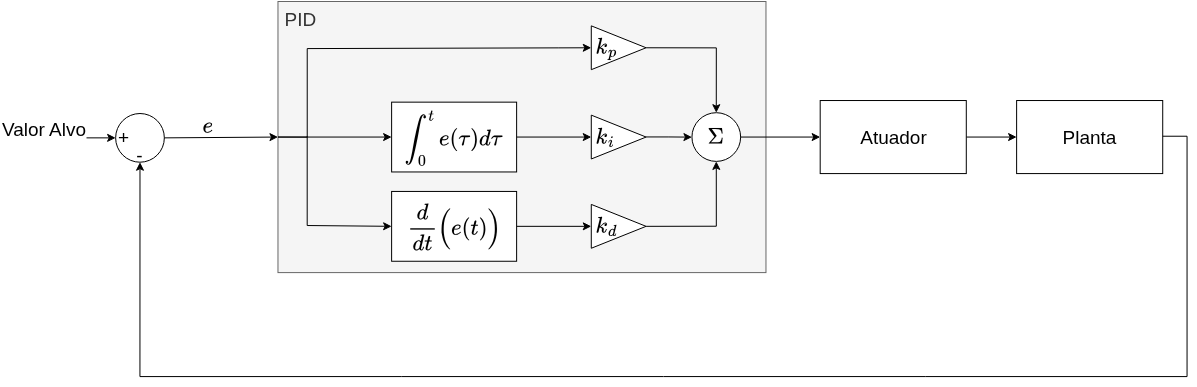
\includegraphics[width=0.9\textwidth]{img/PID_loop (1).png}
    \caption{Malha de Controle - Controlador PID.}
    \label{fig:pid_loop}
\end{figure}
\vspace{10px}


A estrutura de um controlador PID baseia-se no cálculo de uma variável de controle — chamada de 
\emph{esforço de controle} — a partir do erro entre o valor de referência (ou valor desejado) e o valor medido do sistema (fechando, assim, a malha, como podemos ver pela figura \ref{fig:pid_loop}). 
Esse esforço é composto por três termos: proporcional, integral e derivativo, que, combinados, ajustam a resposta do sistema de forma dinâmica \cite{ogata2010modern}.

O termo proporcional atua diretamente sobre o erro instantâneo, aplicando uma correção proporcional à sua magnitude. 
Já o termo integral é responsável por acumular o erro ao longo do tempo, eliminando o erro estacionário e garantindo
que a saída atinja o valor desejado. Por fim, o termo derivativo antecipa o comportamento futuro do erro, reagindo à sua taxa de 
variação, o que contribui para reduzir oscilações e melhorar a estabilidade do sistema \cite{nise2011control}.

Matematicamente, a saída $u(t)$  do controlador PID é expressa por:
\begin{align}
    u(t) = k_pe(t) + k_i\int^t_0e(\tau)d\tau + k_d\frac{d}{dt}\Bigr(e(t)\Bigl),
\end{align}

em que $k_p$, $k_d$, $k_d$ representam, respectivamente, os ganhos proporcional, integral e derivativo. Em implementações digitais — como em sistemas embarcados — essa equação é discretizada, considerando o tempo de amostragem e métodos numéricos adequados para o cálculo da integral e da derivada.

A correta sintonia dos parâmetros é fundamental para o desempenho do controlador. Ajustes inadequados podem resultar em comportamentos indesejados, como oscilações excessivas, lentidão na resposta ou
até instabilidade. Diversos métodos de sintonia, empíricos e analíticos, foram propostos ao longo das décadas, destacando-se o método empírico de Ziegler–Nichols, um dos mais conhecidos
\cite{ziegler1942optimum}.

Dois problemas encontrados de forma recorrente na aplicação do controlador PID em sistemas físicos é a questão de saturação do esforço de controle e o \emph{windup} do integrador. 

O problema de saturação do esforço de controle se dá quando o controlador requer um esforço $u(t)$ maior do que o atuador é capaz de prover. A solução mais simples utilizada é considerar a limitação
do atuador no algoritmo do PID e saturar a saída $u(t)$ antes de ser enviada para o atuador. 

Já o problema de
\emph{windup} consiste no integrador atingir valores muito altos em momentos de erro prolongado por fatores externos, causando uma inflação do
fator integrativo, o que causa oscilações e demora na resposta. Existem diferentes estratégias para evitar a degradação devido a \emph{windup} (chamados de métodos de \emph{anti-windup}), sendo o mais
simples e ainda assim satisfatório o \emph{clamping}, onde o integrador para de integrar o erro se extrapola um limite inferior ou superior \cite{amiri2024antiwindup}.
\newpage

\subsection{Filtros Digitais}
Filtros digitais são elementos fundamentais no processamento de sinais, utilizados para atenuar ruídos, eliminar componentes indesejadas de frequência e realçar informações relevantes em um sinal  \cite{oppenheim1999discrete}. Em sistemas de controle e aplicações embarcadas, o uso de filtros é essencial para garantir medições mais estáveis e precisas, reduzindo a influência de perturbações ou flutuações de sensores.

De modo geral, os filtros digitais podem ser classificados em duas grandes categorias: Filtros de Resposta Finita ao Impulso (FIR, do inglês \emph{Finite Impulse Response}) e Filtros de Resposta Infinita ao Impulso (IIR, do inglês \emph{Infinite Impulse Response}). Essa classificação decorre da forma como o filtro responde a uma entrada do tipo impulso unitário.

Os filtros FIR são caracterizados por uma resposta finita no tempo — ou seja, após um número limitado de amostras, a resposta do filtro torna-se nula. Sua implementação baseia-se apenas em amostras passadas da entrada, sendo, portanto, inerentemente estáveis. Além disso, os filtros FIR podem ser projetados para apresentar uma resposta de fase linear, o que os torna ideais em aplicações onde a preservação da forma de onda é crítica \cite{smith2003digital}.

Por outro lado, os filtros IIR possuem uma resposta teórica infinita, pois dependem não apenas das amostras da entrada, mas também de saídas passadas. Essa característica permite que alcancem respostas em frequência equivalentes às de filtros analógicos com menor ordem e custo computacional reduzido. No entanto, o uso de realimentação pode introduzir riscos de instabilidade e distorções de fase, exigindo um cuidado maior no projeto \cite{proakis2007digital}.

Um caso particular de filtro FIR amplamente utilizado é o filtro de média móvel \cite{mathworks_moving_average_vs_fir}. Esse
filtro calcula a média aritmética de um número fixo de amostras recentes, suavizando variações rápidas no sinal e reduzindo ruídos de alta frequência. Sua forma discreta pode ser representada por:
\begin{align}
    y[n] = \frac{1}{N}\sum_{k=0}^{N-1}x[n-k],
\end{align}

onde $y[n]$ é a saída filtrada, $x[n]$ é a entrada, e $N$ é o tamanho da janela de amostragem.
Embora o filtro de média móvel apresente desempenho limitado na rejeição seletiva de frequências, sua implementação simples — exigindo apenas operações de soma e divisão — e sua estabilidade o tornam
uma escolha recorrente em sistemas embarcados com restrições de processamento e memória \cite{lyons2011understanding}, servindo como uma solução prática para suavização de leituras de sensores antes da aplicação de algoritmos de
controle, como o PID .

\clearpage
\section{Trabalhos Correlatos}\label{chap:projetos_correlatos}
    Nesta seção, serão brevemente revisados trabalhos que implementaram métodos de verificação formal por métodos dedutivos e por métodos de interpretação abstrata em alguma capacidade utilizando a plataforma Frama-c e seus \emph{plugins}. 
    
    Em um primeiro momento, são apresentados projetos que utilizaram tais métodos para garantir a corretude funcional dos softwares desenvolvidos; em seguida são apresentados trabalhos que os utilizaram para garantir a ausência de erros em tempo de execução.
        
    
    
    \subsection{Corretude Funcional}
    
    Métodos formais tem ganho cada vez mais espaço em sistemas críticos de grandes industrias, mas algo que também está impulsionando e disseminando a sua utilização em projetos de natureza aberta é a ferramenta Frama-C open source e seus diversos plug-ins (mais especificamente o WP), que através de métodos dedutivos e da teoria de pré-condição mais fraca possibilitam a verificação formal para programas escritos em C.

    Um exemplo de tal é a iniciativa tomada por Baptiste Pollien de realizar a verificação formal da biblioteca matemática do piloto automático para UAVs chamada de Paparazzi\cite{perrone2016verifying}. Nesse trabalho, o autor analisa duas funções utilizadas para a navegação e planejamento de trajetórias: A função \emph{float\_rmat\_of\_quat}, que recebe como entrada um quaternion normalizado e retorna a matriz de rotação correspondente; e a função inversa \emph{float\_quat\_of\_rmat}. A primeira função conseguiu ter todas as condições de verificação provadas por \emph{solvers} automáticos, enquanto a segunda função não foi capaz de ser provada de forma automática, necessitando então da verificação interativa.

    Esse trabalho reflete o atual estado da arte no que tange solvers automáticos e indica um dos principais desafios da utilização de métodos formais, a necessidade de treinamento específico em métodos formais e em linguagens específicas de assistentes de provas manuais (como COQ) nos casos que a verificação automática falha\cite{yaglamunov2021correctness}.
    
     \subsection{Ausência de Erros em Tempo de Execução}


    Ao plataforma frama-c possui diferentes plug-ins a fim de verificar a ausência dos tipos de erros citados acima. A depender da estrutura e arquitetura do código sendo analisado, entretanto, certos pontos precisam ser levados em consideração no que tange as deficiências de cada ferramenta.

    Como relatado por Baptiste Pollien \cite{perrone2016verifying}, o plug-in RTE é capaz de determinar possíveis ocorrências de erros em tempo de execução em operações aritméticas em funções as quais seus contratos formais não especificam pré-condições que mitiguem tais erros (como especificações de possíveis intervalos para cada variável). Já para programas que utilizam variáveis do tipo \emph{struct}, tal plug-in falha em garantir a ausência de erros por efeito colateral ao realizar operações com seus campos (fato observado também por Vassil Todorov durante sua tese de PhD \cite{todorov2020automotive}).

    A principal alternativa para as limitações citadas é a utilização do plug-in EVA. Ao contrário do plug-in WP/RTE, o EVA (Evolved Value Analysis) é uma ferramenta capaz de calcular sets de possíveis valores para variáveis em programas analisados por métodos de interpretação abstrata\cite{framaC_eva_manual}, a partir dos quais é capaz de verificar a ausência (ou possível presença) de erros em casos mais complexos. 


\clearpage
\section{Metodologia e Ferramentas}\label{chap:metodologia}

Nesta seção, são apresentadas as ferramentas e especificações utilizados para a análise e verificação de código fonte na linguagem C, assim como os procedimentos e etapas para atingir os objetivos de garantia de corretude funcional e ausência de erros em tempo de execução.

\subsection{Ferramentas}
\subsubsection{Frama-C}
Frama-C (\emph{Framework for Modular Analysis of C Code}) é uma plataforma modular, portada tanto para sistemas baseados em Unix quanto para Windows, criada pela CEA List e Inria, com foco na análise, em diferentes esferas, de códigos fontes escritos em C. A sua modularidade vem a partir da sua arquitetura baseada em \emph{plugins}, que estendem sua funcionalidade em diferentes campos, sendo alguns deles: Análise de códigos desconhecidos, gerador de especificação, métodos formais e transformação de código.

\begin{figure}[h]
    \centering
    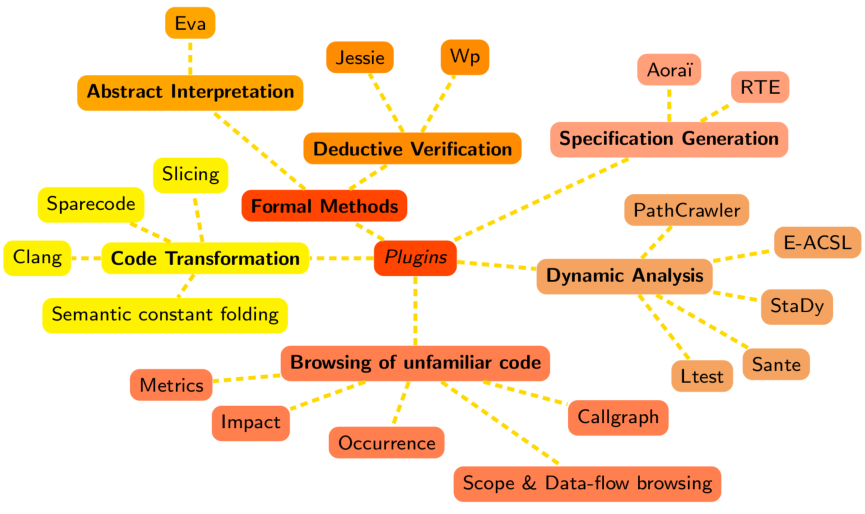
\includegraphics[width=0.6\linewidth]{img/frama_c_plugins.png}
    \caption{Diferentes \emph{plugins} do FramaC. Fonte: \cite{blanchard2020introduction}}
    \label{fig:enter-label}
\end{figure}
\vspace{5px}

É possível utilizar a ferramenta em seu modo com interface gráfica (\emph{frama-c-gui}), como demonstrado pela figura \ref{fig:frama_c_gui}, onde o usuário é capaz de ver (mas não é capaz de editar) os códigos fontes em análise, assim como verificar os status das análises dos diferentes \emph{plugins}. 

\vspace{10px}
\begin{figure}[h]
    \centering
    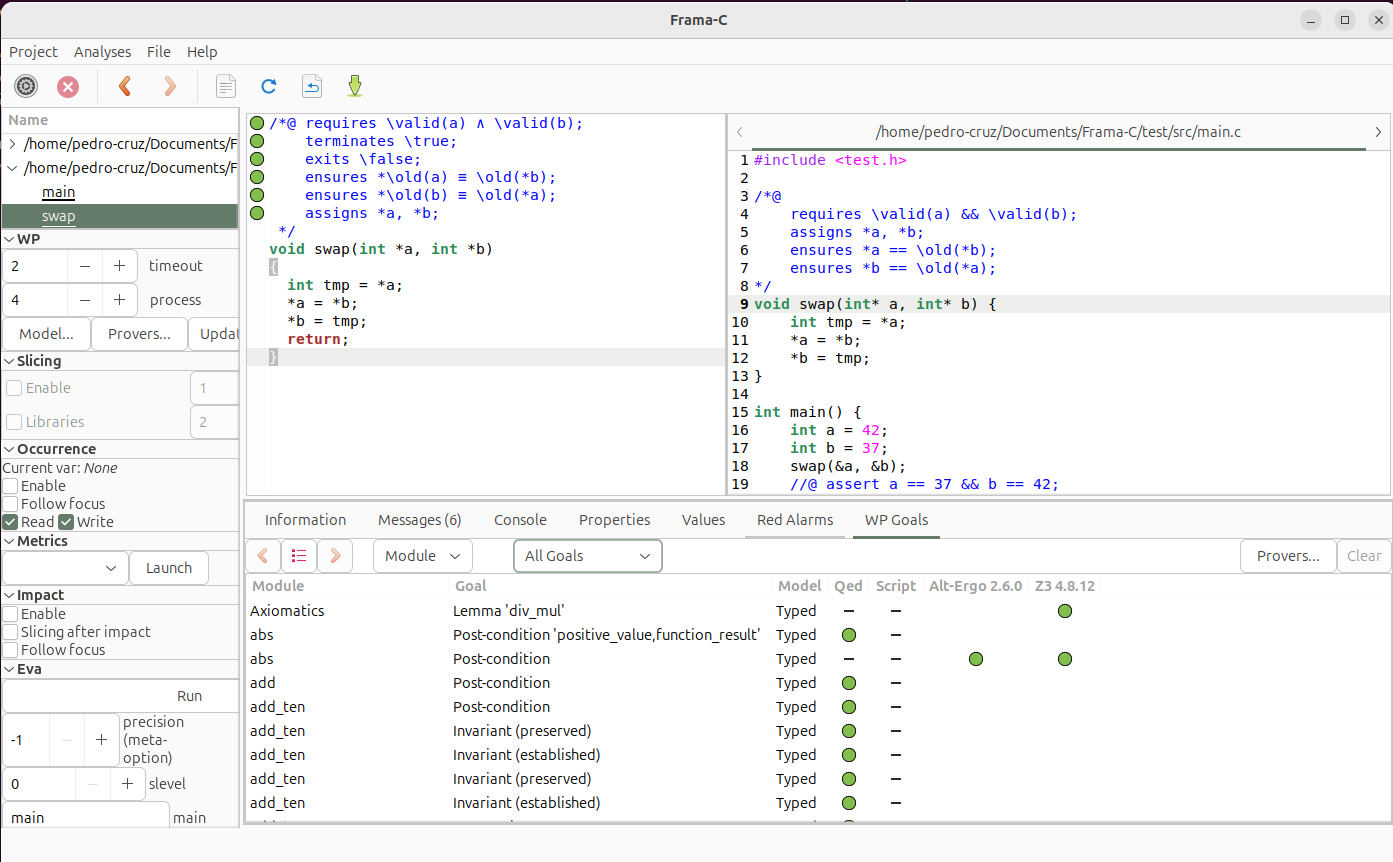
\includegraphics[width=0.75\linewidth]{img/frama_c_gui.png}
    \caption{Interface Gráfica Frama-C.}
    \label{fig:frama_c_gui}
\end{figure}

Uma outra alternativa é a utilização da versão de terminal (chamada de \emph{cli}) da ferramenta Frama-C, como mostrada na figura \ref{fig:frama_c_cli}, onde todos os status são expostos diretamente no terminal. 

\vspace{10px}
\begin{figure}[h]
    \centering
    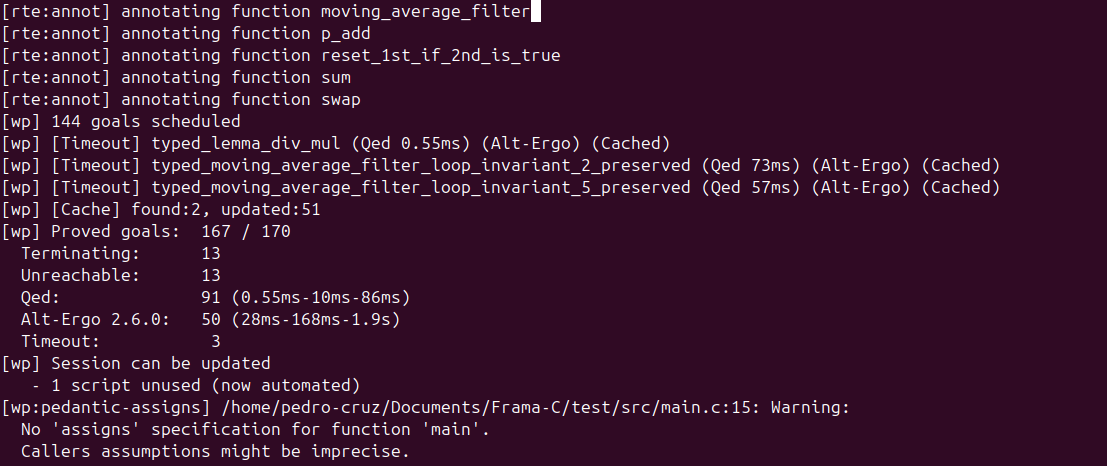
\includegraphics[width=0.75\linewidth]{img/frama_c_cli.png}
    \caption{Interface por Terminal Frama-C.}
    \label{fig:frama_c_cli}
\end{figure}

\subsubsection{ACSL}
A linguagem ACSL (ANSI/ISO C Specification Language), lida como (``\emph{Axel}"), é uma linguagem formal desenvolvida para especificar o comportamento de programas escritos em C nos próprios arquivos fonte em forma de comentários, seguindo um padrão similiar o de anotação Doxygen, sendo no formato \emph{/*@ ... */}. Inspirada pela Java Modeling Language (JML) e pelo analisador de código Caduceus, ACSL foi projetada com o objetivo de descrever propriedades funcionais e construções específicas da linguagem C (\emph{e.g} como validade de ponteiros) de maneira precisa e verificável. Seu foco principal está na definição de contratos de função — ou seja, na especificação formal de pré-condições, pós-condições e invariantes relacionadas ao comportamento esperado de funções. Diferentemente de anotações informais ou verificações em tempo de execução, ACSL permite que essas propriedades sejam verificadas estaticamente, tornando-se uma base sólida para a aplicação de técnicas de verificação formal em sistemas críticos \cite{framaCacsl}.

A seguir são apresentadas as principais construções pertencentes à linguagem ACSL que são suportadas pela plataforma Frama-C.

\paragraph{Precondições (\texttt{requires})} 
Indicam as condições que devem ser verdadeiras antes da execução de uma função. São hipóteses assumidas como válidas durante a verificação.
\begin{lstlisting}[language=C]
                            /*@ requires x > 0; */
                            void function(int x){...}
\end{lstlisting}

O exemplo acima define que a função deve ser chamada apenas se \texttt{x > 0}.

\paragraph{Validade de Ponteiros (\texttt{\textbackslash valid} e \texttt{\textbackslash valid\_read})} 

Um dos principais desafios ao trabalhar com a linguagem C é a manipulação segura de ponteiros. ACSL fornece predicados especiais para especificar e verificar a validade de regiões de memória apontadas:

\begin{itemize}
    \item \texttt{\textbackslash valid(p)} — Indica que o ponteiro \texttt{p} aponta para uma região de memória válida para leitura \textbf{e} escrita.
    \item \texttt{\textbackslash valid(p + (0 .. n-1))} — Indica que os \texttt{n} primeiros elementos a partir de \texttt{p} são válidos.
    \item \texttt{\textbackslash valid\_read(p)} — Indica que \texttt{p} aponta para uma região de memória válida apenas para leitura.
\end{itemize}

\paragraph{Pós-condições (\texttt{ensures})} 
Especificam as propriedades que devem ser verdadeiras ao término da função, desde que as precondições tenham sido respeitadas e o código termine. O valor de retorno é referenciado com \texttt{\textbackslash result}.
\begin{lstlisting}[language=C]
                            ...
                            /*@ ensures \result >= 0; */
                            int function(){...}
\end{lstlisting}

\paragraph{Rótulos e Estados Antigos (\texttt{at}, \texttt{old})} 
Rótulos permitem referenciar valores de variáveis em diferentes momentos da execução. \texttt{\textbackslash old} refere-se ao valor de uma expressão antes da execução da função.
\begin{lstlisting}[language=C]
                            /*@ ensures *a == \old(*b); */
\end{lstlisting}
Também é possível utilizar rótulos personalizados com \texttt{label} e acessá-los com \texttt{\textbackslash at(expr, Label)}.

\paragraph{Invariantes de Laço (\texttt{loop invariant})} 
São propriedades que devem permanecer verdadeiras a cada iteração de um laço. Essenciais para comprovar a correção parcial de loops.
\begin{lstlisting}[language=C]
                            /*@ loop invariant 0 <= i <= n; */
\end{lstlisting}

\paragraph{Atribuições em Laços (\texttt{loop assigns})} 
Define quais variáveis podem ser modificadas dentro do laço. Garante que outras variáveis permanecem inalteradas.
\begin{lstlisting}[language=C]
                            /*@ loop assigns i, sum; */
\end{lstlisting}

\paragraph{Variação de Laço (\texttt{loop variant})} 
Expressão natural que deve decrescer a cada iteração, usada para provar a terminação do laço (a fim de auxiliar solvers na prova de correção total).
\begin{lstlisting}[language=C]
                            /*@ loop variant n - i; */
\end{lstlisting}

\paragraph{Código Fantasma (\texttt{ghost})} 
São variáveis ou instruções em C usadas exclusivamente para fins de verificação, utilizados para tornar explicitas relações e estados durante a execução do programa que seriam somente implicitas e difíceis dos \emph{solvers} de analisarem. Não impactam a execução real do programa.
\begin{lstlisting}[language=C]
                            /*@ ghost int acc = 0; */
\end{lstlisting}

\paragraph{Funções e Predicados Lógicos}
ACSL permite definir abstrações matemáticas com funções puramente lógicas (que não são restritas, por exemplo, a tipos de variáveis de C como int e float, mas sim utilizam construções matematicas como \texttt{real} e \texttt{integer}) através da sintaxe \texttt{logic}, utilizadas para a especificação de conceitos mais abstratos e complexos, assim como a definição de \texttt{predicate} para expressar propriedades reutilizáveis.
\begin{lstlisting}[language=C]
        /*@ 
            logic integer abs(int x) = (x >= 0) ? x : -x; 
            predicate valid_array_r(int* array, unsigned int length) =
                \valid_read(array+(0..length-1)) && 0<=length<=INT_MAX;
        */
\end{lstlisting}

\paragraph{Lemas}
São proposições auxiliares sobre predicados ou funções lógicas, escritas com a palavra-chave \texttt{lemma}, utilizadas para ajudar os provadores automáticos durante as provas.
\begin{lstlisting}[language=C]
                    /*@ lemma abs_pos: \forall int x; abs(x) >= 0; */
\end{lstlisting}

\paragraph{Comportamentos Múltiplos (\texttt{behavior})} 
Permite descrever diferentes cenários de execução com suposições distintas (\texttt{assumes}) e suas respectivas garantias (\texttt{ensures}).
\begin{lstlisting}[language=C]
                            /*@ 
                              behavior positive:
                                assumes x > 0;
                                ensures \result > 0;

                              behavior zero:
                                assumes x == 0;
                                ensures \result == 0;
                            */
\end{lstlisting}
O uso de comportamentos facilita a modularização de especificações complexas.

\paragraph{Definições Axiomáticas (\texttt{axiomatic})}

Definições axiomáticas são usadas para introduzir conceitos lógicos abstratos — como funções, predicados e lemas — que não necessariamente possuem implementação concreta no código C, mas que são úteis para a construção e prova de especificações formais. Elas permitem descrever propriedades gerais, muitas vezes matemáticas, que o sistema pode assumir como verdadeiras e não necessitam que \emph{solvers} os provem.

A construção \texttt{axiomatic} é composta por:

\begin{itemize}
    \item \texttt{logic} functions ou predicados;
    \item \texttt{axiom}s — proposições assumidas como verdadeiras;
    \item \texttt{lemma}s — propriedades a serem provadas ou utilizadas em provas.
\end{itemize}

\begin{lstlisting}[language=C]
        /*@ axiomatic lt_plus_lt{ 
                axiom always_true_lt_plus_lt: 
                \forall integer i, j; i < j ==> i+1 < j+1 ;
                }
        */ 
\end{lstlisting}

Essas construções formam a base para a escrita de especificações formais em C com o ACSL, viabilizando a verificação automática por meio do Frama-C e seu plugin WP.



\subsubsection{Plugins - WP e EVA}

O plugin \texttt{WP} (\emph{Weakest Precondition}) é um verificador dedutivo. Ele implementa a técnica de cálculo da pré-condição mais fraca, formulada por Edsger Dijkstra e descrita na seção \ref{sec:wp}, com o objetivo de provar que o código C cumpre a especificação dada em anotações ACSL.

A partir das anotações ACSL e do código-fonte, o WP gera condições de verificação (\emph{verification conditions} — VCs), que são fórmulas lógicas. Essas fórmulas precisam ser válidas (ou satisfazíveis) para garantir que o código respeita a especificação. 

O processo de verificação pode ser realizado de forma:
\begin{itemize}
    \item Manual: Utilizando assistentes de prova interativos como o \textit{Coq};
    \item Automática: Por meio de \emph{solvers} SMT(\textit{Satisfiability Modulo Theories}).
\end{itemize}

Neste trabalho, visa-se utilizar a abordagem automática, especialmente com o Alt-Ergo, um \emph{solver} SMT desenvolvido inicialmente pelo Laboratoire de Recherche en Informatique d’Orsay, atualmente mantido pela OCamlPro, além dos \emph{solvers} Z3 e CVC5, por meio da integração com o Why3.

Já o \emph{plugin} \texttt{EVA} (\textit{E-Value Analysis}) realiza análise abstrata de código C, com foco na detecção de possíveis erros de execução em tempo de execução (RTEs), como:
\begin{itemize}
    \item Acesso fora dos limites de um vetor;
    \item Ponteiros inválidos ou não inicializados;
    \item Divisões por zero;
    \item \emph{Overflow} e \emph{underflow} de inteiros.
\end{itemize}

Enquanto o WP prova propriedades baseadas em uma especificação formal, o EVA trabalha com uma abordagem conservadora de interpretação abstrata, explorando todos os caminhos possíveis de execução, sem necessidade de especificações formais do usuário.


\newpage
\subsection{Procedimento de Verificação}
O procedimento para a verificação utilizado foi baseado no utilizado por Rovedy Aparecida Busquim e Silva em \cite{silva2016formal}, onde ocorre o preparo do ambiente e dos
códigos fontes que serão analisados, posteriormente são feitas, de forma iterativa, a análise de erros em tempo de execução (RTE) e por fim são escritos os contratos formais e 
quaisquer deduções auxiliares para a verificação funcional.

\vspace{10px}
\begin{figure}[h!]
    \centering
    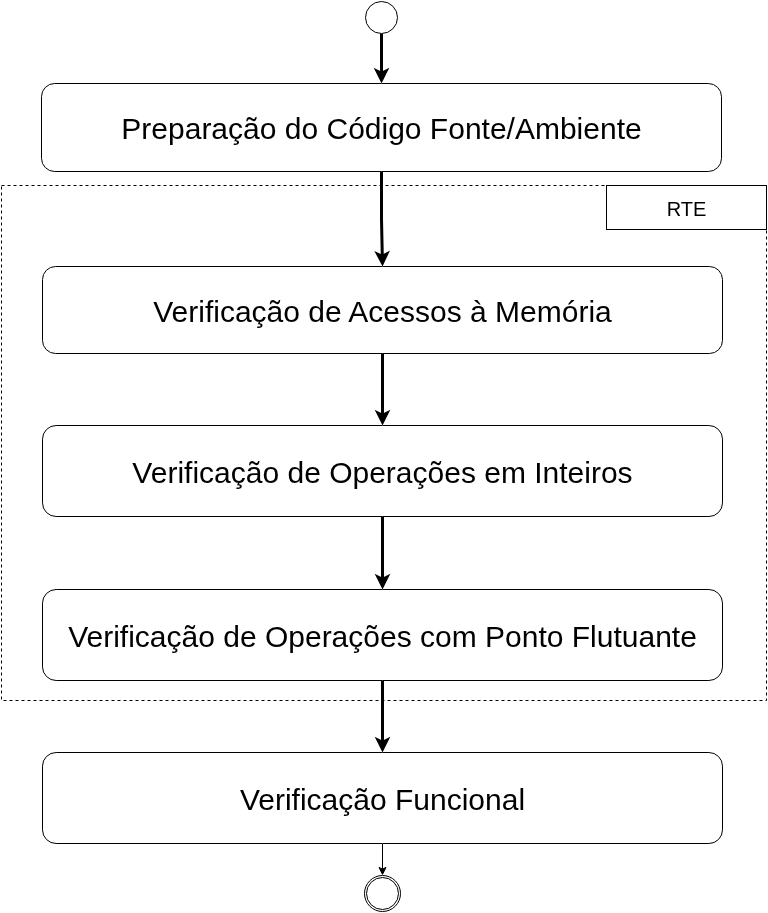
\includegraphics[width=.35\textwidth]{img/fluxograma.png}
    \caption{Fluxo de Verificação.}
\end{figure}
\vspace{10px}

\subsubsection{Preparação do Código Fonte e Ambiente}
\subsubsection{Verificação de Erros em Tempo de Execução}
\subsubsection{Verificação Funcional}

\clearpage
\section{Resultados}\label{chap:resultados}

\newpage
\printbibliography[title={Referências}]

\end{document}